\section{Gorizontga nisbatan burchak ostida otilgan jismning harakati}



\begin{enumerate}

\item Gorizontga burchak ostida otilgan jismning traektoriyasi qanday bo‘ladi? Havoning qarshiligini hisobga olmang.
\begin{enumerate}[label=\Alph*)]
\item ellips.
\item gorizontga qiya to‘g‘ri chiziq.
\item aylana.
\item parabola.
\end{enumerate}

\item Rasmda gorizontga $\alpha$ burchak ostida $v$ tezlik bilan otilgan jismning harakat traektoriyasi ko‘rsatilgan. Rasmda ko‘rsatilgan vektorlardan qaysi biri jismning A nuqtadagi tezlanishi yo‘nalishini ko‘rsatadi?
\begin{center}
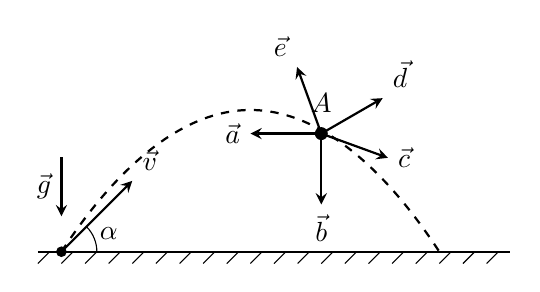
\begin{tikzpicture}[scale=1.5, >=stealth]
  % Ground line
  \draw[thick] (0,0) -- (4,0);
  \foreach \x in {0.1, 0.3, 0.5, 0.7, 0.9, 1.1, 1.3, 1.5, 1.7, 1.9, 2.1, 2.3, 2.5, 2.7, 2.9, 3.1, 3.3, 3.5, 3.7, 3.9} {
    \draw (\x, 0) -- (\x-0.1, -0.1);
  }
  
  % Trajectory (parabola)
  \draw[thick, dashed] (0.2,0) parabola bend (1.8,1.2) (3.4,0);
  
  % Launch angle and velocity
  \draw[fill=black] (0.2,0) circle (0.04);
  \draw[->, thick] (0.2,0) -- (0.8, 0.6) node[above right] {$\vec{v}$};
  \draw (0.5,0) arc (0:45:0.3);
  \node at (0.6, 0.15) {$\alpha$};
  
  % Point A
  \coordinate (A) at (2.4, 1);
  \draw[fill=black] (A) circle (0.05) node[above=4pt] {$A$};
  
  % Vectors from A
  \draw[->, thick] (A) -- +(180:0.6) node[left] {$\vec{a}$};
  \draw[->, thick] (A) -- +(270:0.6) node[below] {$\vec{b}$};
  \draw[->, thick] (A) -- +(340:0.6) node[right] {$\vec{c}$};
  \draw[->, thick] (A) -- +(30:0.6) node[above right] {$\vec{d}$};
  \draw[->, thick] (A) -- +(110:0.6) node[above left] {$\vec{e}$};
  
  % Vector g at launch
  \draw[->, thick] (0.2, 0.8) -- (0.2, 0.3) node[midway, left] {$\vec{g}$};
\end{tikzpicture}
\end{center}
\begin{enumerate}[label=\Alph*)]
\item a.
\item b.
\item c.
\item d.
\end{enumerate}

\item Gorizontga burchak ostida otilgan jismning tezlanishi qanday bo‘ladi?
\begin{enumerate}[label=\Alph*)]
\item nolga teng.
\item $g$, pastga yo‘nalgan.
\item $g$, yuqoriga yo‘nalgan.
\item $g$, tezlik vektori bo‘ylab yo‘nalgan.
\end{enumerate}

\item Sharcha gorizontga $30^\circ$ burchak ostida 30 m/s boshlang‘ich tezlik bilan otildi. Boshlang‘ich tezlik vektorining gorizontal va vertikal tashkil etuvchilari qanday (m/s)?
\begin{enumerate}[label=\Alph*)]
\item 26; 15.
\item 15; 26.
\item 15; 15.
\item 26; 26.
\end{enumerate}

\item Jism gorizontga $30^\circ$ burchak ostida 20 m/s boshlang‘ich tezlik bilan otildi. Harakatning 0,3-sekund oxiridagi tezlik vektorining gorizontal va vertikal tashkil etuvchilari qanday (m/s)? $\sin30^\circ=0,5$; $\cos30^\circ=0,87$.
\begin{enumerate}[label=\Alph*)]
\item 10 va 17,3.
\item 17,3 va 10.
\item 17,3 va 7.
\item 17,3 va 17,3.
\end{enumerate}


\item Gorizontga $45^\circ$ burchak ostida otilgan jismning 2 s dan keyin tezligi minimal qiymatga erishgan bo‘lsa, u qanday tezlik bilan otilgan (m/s)? $g=10$ m/s$^2$.
\begin{enumerate}[label=\Alph*)]
\item 20.
\item $10\sqrt{2}$.
\item $20\sqrt{2}$.
\item 40.
\end{enumerate}

\item Gorizontga $30^\circ$ burchak ostida 20 m/s tezlik bilan otilgan jismning tezlik vektori qancha vaqtdan so‘ng gorizont bilan $0^\circ$ burchak hosil qiladi (s)? $g=10$ m/s$^2$.
\begin{enumerate}[label=\Alph*)]
\item 2.
\item 3.
\item 4.
\item 1.
\end{enumerate}

\item Gorizontga burchak ostida 10 m/s tezlik bilan otilgan jismning uchish davomidagi minimal tezligi 6 m/s bo‘lsa, uning uchish vaqti qanday (s) bo‘ladi? $g=10$ m/s$^2$.
\begin{enumerate}[label=\Alph*)]
\item 1,6.
\item 0,8.
\item 0,6.
\item 1,2.
\end{enumerate}

\item Gorizontga burchak ostida 25 m/s tezlik bilan otilgan jism 4 s da yerga qaytib tushdi. Uning uchish davomidagi minimal tezligi qanday (m/s).
\begin{enumerate}[label=\Alph*)]
\item 15.
\item 10.
\item 20.
\item 25.
\end{enumerate}

\item Zambarakdan gorizontga burchak ostida uchib chiqqan snaryad 12 s uchgan. Snaryad ko‘tarilgan eng yuqori balandlik qanday (m)?
\begin{enumerate}[label=\Alph*)]
\item 170.
\item 180.
\item 190.
\item 200.
\end{enumerate}

\item Ikki o‘quvchi bir-biriga to‘p otib o‘ynamoqda. Agar to‘p birinchi o‘quvchidan ikkinchi o‘quvchiga 2 s vaqt mobaynida yetib borsa, to‘p o‘yin vaqtida qanday eng yuqori balandlikka (m) erishadi? $g=10$ m/s$^2$.
\begin{enumerate}[label=\Alph*)]
\item 1.
\item 2.
\item 3.
\item 5.
\end{enumerate}

\item Zambarakdan gorizontga nisbatan burchak ostida otilgan snaryad 20 m balandlikka ko‘tarildi. Uning uchish vaqtini toping (s). $g=10$ m/s$^2$.
\begin{enumerate}[label=\Alph*)]
\item 10.
\item 20.
\item 1.
\item 4.
\end{enumerate}



\item Gorizontga nisbatan $45^\circ$ burchak ostida 10 m/s tezlik bilan otilgan jism 8 m naridagi vertikal devorga mutloq elastik urilib qaytdi va yerga tushdi. Jism otilish nuqtasidan qanday masofada tushadi (m)? $g=10$ m/s$^2$.
\begin{center}
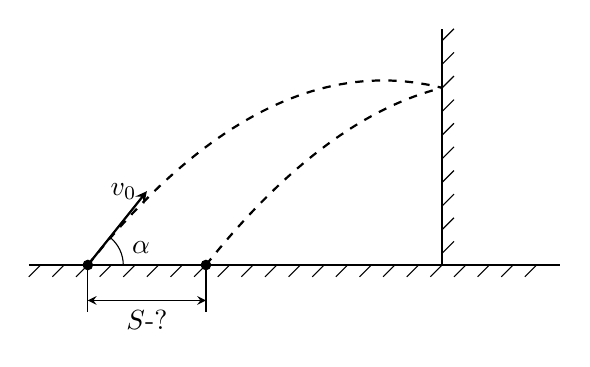
\begin{tikzpicture}[scale=1.5, >=stealth]
  % Ground line
  \draw[thick] (-0.5,0) -- (4,0);
  \foreach \x in {-0.4, -0.2, 0, 0.2, 0.4, 0.6, 0.8, 1, 1.2, 1.4, 1.6, 1.8, 2, 2.2, 2.4, 2.6, 2.8, 3, 3.2, 3.4, 3.6, 3.8} {
    \draw (\x, 0) -- (\x-0.1, -0.1);
  }
  
  % Vertical Wall at x=3.0
  \draw[thick] (3.0,0) -- (3.0,2.0);
  \foreach \y in {0.1, 0.3, 0.5, 0.7, 0.9, 1.1, 1.3, 1.5, 1.7, 1.9} {
    \draw (3.0,\y) -- (3.1,\y+0.1);
  }
  
  % Launch Point at x=0
  \draw[fill=black] (0,0) circle (0.04);
  
  % Incident Trajectory (parabola to wall)
  \draw[thick, dashed, domain=0:3.0, samples=50] plot (\x, {1.25*\x - 0.25*\x*\x});
  
  % Reflected Trajectory
  \draw[thick, dashed, domain=1.0:3.0, samples=50] plot (\x, {0.25*(6-\x)*(\x-1)});
  
  % Landing points
  \draw[fill=black] (1.0,0) circle (0.04);
  
  % Labels
  \draw[->, thick] (0,0) -- (0.5,0.625) node[left] {$v_0$};
  \draw (0.3,0) arc (0:51:0.3);
  \node at (0.45,0.15) {$\alpha$};
  
  % Distance helper
  \draw[<->, thin] (0,-0.3) -- (1.0,-0.3) node[midway, below] {$S$-?};
  \draw[thin] (0,0) -- (0,-0.4);
  \draw[thin] (1.0,0) -- (1.0,-0.4);
\end{tikzpicture}
\end{center}
\begin{enumerate}[label=\Alph*)]
\item 6.
\item 4.
\item 8.
\item 2.
\end{enumerate}

\item 20 m/s tezlik bilan gorizontga burchak ostida otilgan jismning maksimal ko‘tarilish balandligi 15 m bo‘lsa, uning uchish davomidagi minimal tezligi necha m/s bo‘lgan?
\begin{enumerate}[label=\Alph*)]
\item 20.
\item 15.
\item 10.
\item 5.
\end{enumerate}

\item Gorizontga burchak ostida otilgan jismning uchish davomidagi minimal tezligi 16 m/s, uchish vaqti esa 2,4 s bo‘lsa, u qanday (m/s) tezlik bilan otilgan?
\begin{enumerate}[label=\Alph*)]
\item 35.
\item 30.
\item 24.
\item 20.
\end{enumerate}

\item Gorizontga burchak ostida 20 m/s tezlik bilan otilgan jismning uchish davomidagi minimal tezligi 10 m/s bo‘lsa, u necha metr balandlikka ko‘tarilgan? $g=10$ m/s$^2$.
\begin{enumerate}[label=\Alph*)]
\item 5.
\item 25.
\item 20.
\item 15.
\end{enumerate}

\item Bir vaqtning o‘zida ikkita jism bir nuqtadan bir xil 10 m/s boshlang‘ich tezlik bilan biri vertikal va ikkinchisi gorizontga nisbatan $30^\circ$ burchak ostida yuqoriga otildi. 1 s dan keyin jismlar orasidagi masofa qanday bo‘ladi (m)?
\begin{enumerate}[label=\Alph*)]
\item 5.
\item 7,4.
\item 10.
\item 12,5.
\end{enumerate}



\item Uchish uzoqligi ko‘tarilish balandligidan 4 marta ortiq bo‘lishi uchun jism gorizontga qanday burchak ostida otilishi kerak?
\begin{enumerate}[label=\Alph*)]
\item arctg3.
\item arctg2.
\item $30^\circ$.
\item $45^\circ$.
\end{enumerate}

\item Gorizontga $45^\circ$ burchak ostida otilgan disk 20 m ko‘tarildi. Uning uchish uzoqligi qanday (m)?
\begin{enumerate}[label=\Alph*)]
\item 20.
\item 40.
\item 80.
\item 160.
\end{enumerate}

\item Gorizontga $\alpha$ burchak ostida otilgan jismning harakati quyida tasvirlangan. $h/x$ ning qiymatini toping.
\begin{center}
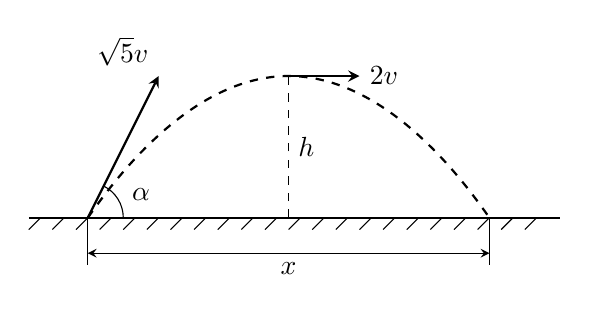
\begin{tikzpicture}[scale=1.5, >=stealth]
  % Ground line
  \draw[thick] (-0.5,0) -- (4,0);
  \foreach \x in {-0.4, -0.2, 0, 0.2, 0.4, 0.6, 0.8, 1, 1.2, 1.4, 1.6, 1.8, 2, 2.2, 2.4, 2.6, 2.8, 3, 3.2, 3.4, 3.6, 3.8} {
    \draw (\x, 0) -- (\x-0.1, -0.1);
  }
  
  % Trajectory
  \draw[thick, dashed] (0,0) parabola bend (1.7,1.2) (3.4,0);
  
  % Launch vector
  \draw[->, thick] (0,0) -- (0.6, 1.2) node[above left] {$\sqrt{5}v$};
  \draw (0.3,0) arc (0:63.4:0.3);
  \node at (0.45,0.2) {$\alpha$};
  
  % Height h
  \draw[dashed] (1.7,0) -- (1.7,1.2);
  \node[right] at (1.7,0.6) {$h$};
  
  % Peak velocity vector
  \draw[->, thick] (1.7,1.2) -- (2.3,1.2) node[right] {$2v$};
  
  % Range x helper
  \draw[<->, thin] (0,-0.3) -- (3.4,-0.3) node[midway, below] {$x$};
  \draw[thin] (0,0) -- (0,-0.4);
  \draw[thin] (3.4,0) -- (3.4,-0.4);
\end{tikzpicture}
\end{center}
\begin{enumerate}[label=\Alph*)]
\item 1/3.
\item 1/4.
\item 1/8.
\item 3/8.
\end{enumerate}

\item Bir nuqtadan ikkita jism gorizontga burchak ostida rasmdagi kabi otildi. Rasmdagi ma’lumotlardan foydalanib, $h_1/h_2$ nisbatni toping (m). $\alpha=37^\circ$.
\begin{center}
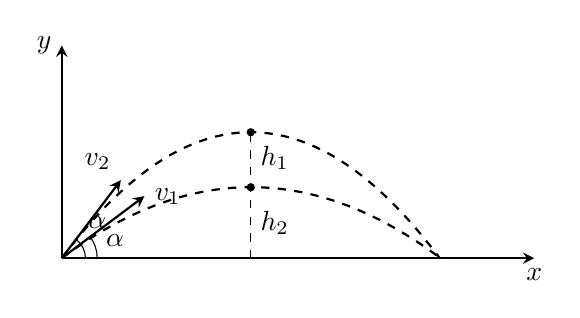
\begin{tikzpicture}[scale=1.5, >=stealth]
  % Axes
  \draw[->, thick] (0,0) -- (0,1.8) node[left] {$y$};
  \draw[->, thick] (0,0) -- (4,0) node[below] {$x$};
  
  % Two trajectories landing at x=3.2
  \draw[thick, dashed, domain=0:3.2, samples=50] plot (\x, {1.333*\x - 0.4166*\x*\x});
  \draw[thick, dashed, domain=0:3.2, samples=50] plot (\x, {0.75*\x - 0.234*\x*\x});
  
  % Peak indicators
  \draw[dashed] (1.6,0) -- (1.6,1.066);
  \draw[fill=black] (1.6,1.066) circle (0.03);
  \draw[fill=black] (1.6,0.6) circle (0.03);
  \node[right] at (1.6, 0.85) {$h_1$};
  \node[right] at (1.6, 0.3) {$h_2$};
  
  % Launch vectors
  \draw[->, thick] (0,0) -- (0.5, 0.66) node[above left] {$v_2$};
  \draw[->, thick] (0,0) -- (0.7, 0.525) node[right] {$v_1$};
  
  % Angles
  \draw (0.3,0) arc (0:37:0.3);
  \node at (0.45,0.15) {$\alpha$};
  
  \draw (0.2,0) arc (0:53:0.2);
  \node at (0.3,0.3) {$\alpha$};
\end{tikzpicture}
\end{center}
\begin{enumerate}[label=\Alph*)]
\item 4/5.
\item 5/7.
\item 7/9.
\item 1.
\end{enumerate}



\item Jism gorizontga $60^\circ$ burchak ostida 20 m/s tezlik bilan otildi. Jism maksimal balandlikka ko‘tarilgan nuqtada traektoriyaning egrilik radiusi qanday bo‘ladi (m)?
\begin{enumerate}[label=\Alph*)]
\item 5.
\item 10.
\item 20.
\item 40.
\end{enumerate}

\item Gorizontga burchak ostida otilgan jismning ko‘tarilish balandligi 3 m, traektoriyaning eng yuqori nuqtasidagi egrilik radiusi 2 m bo‘lsa, jism gorizontga qanday burchak ostida otilgan?
\begin{enumerate}[label=\Alph*)]
\item $45^\circ$.
\item $75^\circ$.
\item $60^\circ$.
\item $30^\circ$.
\end{enumerate}

\item Gorizontga burchak ostida otilgan jism harakat traektoriyasining eng yuqori nuqtasining egrilik radiusi jismning maksimal ko‘tarilish balandligiga teng bo‘lsa, jismning otilish burchagini toping. Erkin tushish tezlanishini 10 m/s$^2$ deb oling.
\begin{enumerate}[label=\Alph*)]
\item $\text{arctg}\sqrt{2}$.
\item $\text{arctg}4$.
\item $\text{arctg}2$.
\item $45^\circ$.
\end{enumerate}

\item Jism gorizontga $60^\circ$ burchak ostida 20 m/s tezlik bilan otildi. Necha sekunddan so‘ng tezlik vektori gorizont bilan $45^\circ$ burchak hosil qiladi? $\sqrt{3}\approx 1,73$.
\begin{enumerate}[label=\Alph*)]
\item 1 va 2.
\item 0,73 va 2,73.
\item 3.
\item 1 va 2,8.
\end{enumerate}

\end{enumerate}



\begin{table}[!ht]
\centering
\begin{tabular}{|c|c|c|c|c|c|c|c|c|c|c|}
\hline
1d & 2b & 3b & 4a & 5c & 6c & 7d & 8a & 9a & 10b & 11d \\ \hline
12d & 13a & 14c & 15d & 16d & 17c & 18d & 19c & 20c & 21c & 22b \\ \hline
23c & 24a & 25b & & & & & & & & \\ \hline
\end{tabular}
\end{table}